\documentclass[a4paper,11pt]{article}
\pagenumbering{gobble}
\usepackage[T1]{fontenc} % codifica dei font
\usepackage[utf8]{inputenc} % lettere accentate da tastiera
\usepackage[english]{babel} % lingua del documento

\usepackage{listings}
\usepackage{geometry}
\usepackage{hyperref}
\usepackage{amsmath}
\usepackage{graphicx}

\begin{document}

\author{Roberto Garza. Reviewed by Khoa Nguyen}
\date{\today}
\title{Step-by-Step Patient Specific VTA Estimation}
\iffalse \date{\vspace{-5ex}} \fi

\maketitle

%__________________________________________________________________________________________________
%__________________________________________________________________________________________________
\section{Purpose}

The present document aims at instructing the user about how to estimate a Volume of Tissue Activated (VTA) taking into account anisotropy information. This is inferred from patient-specific diffusion data and used to obtain the conduction model.

%__________________________________________________________________________________________________
%__________________________________________________________________________________________________
\section{What is needed}

%__________________________________________________________________________________________________
\subsection{Software}

The pipeline described here requires the following softwares:
\begin{itemize}
\item Matlab environmet (download it \href{https://it.mathworks.com/downloads/}{here});
\item the proper version of LEAD-DBS (download it \href{https://github.com/CaprioloSaggio/leaddbs}{here});
\item a Window Subsystem for Linux (in case not working with a Unix-based Operating System yet);
\item FSL (download it \href{https://fsl.fmrib.ox.ac.uk/fsldownloads_registration}{here});
\item MRTRIX (download it \href{https://www.mrtrix.org/download/}{here});
\item ANTS (download it \href{https://github.com/ANTsX/ANTs}{here}).
\end{itemize}

%__________________________________________________________________________________________________
\subsection{Data}

The following data are needed to carry out the whole pipeline:
\begin{itemize}
\item LEAD-DBS data (they can be found in the "Step-by-Step Preprocessing and lead reconstruction with LEAD-DBS" instructions);
\item a diffusion image in DICOM format, possibly acquired witht the same orientation of the reference structural image.
\end{itemize}

%__________________________________________________________________________________________________
%__________________________________________________________________________________________________
\section{LEAD-DBS}

First of all, it is necessary to reconstruct the leads. For this purpose, detailed instructions can be found in "Step-by-Step Preprocessing and lead reconstruction with LEAD-DBS" document\footnote{It can be downloaded at \url{https://github.com/CaprioloSaggio/anisoVTApreprocessing/blob/main/WI_Lead-DBSReconstruction.pdf}}. During this step the reference structural image is altered and we then have always to consider this version of the file. Specifically, Lead-DBS changes the reference structural volume (e.g. anat\_t1) to convert from scanner space to MNI patient space. The raw files are saved as \emph{raw\_<structural\_image\_name>} (e.g. raw\_anat\_t1).

%__________________________________________________________________________________________________
%__________________________________________________________________________________________________
\section{DW-MRI Image Preprocessing}

%__________________________________________________________________________________________________
\subsection{MRTRIX Image Correction}

The following steps regard a single acquisition. In case the images of interest are splitted in more than one acquisition (i.e. a folder containing coherent dicom files describing a 3D or 4D image), the steps described in the present section must be repeated for all of them and then merged in a single 4D image. The next sections are applicable with conditions dependent on how data are organized in the specific case. 

\begin{itemize}

\item convert from DICOM to .mif, we assume here that the DICOM files are contained inside a folder called DICOM:
\begin{lstlisting}[language=bash]
$ mrconvert DICOM dti_raw.mif 
\end{lstlisting}

\item export bvecs and bvals as text files from images:
\begin{lstlisting}[language=bash]
$ mrinfo dti_raw.mif -export_grad_fsl bvecs bvals
\end{lstlisting}

\item apply denoising, according to the assumption on the nature of noise in this 
algorithm, this must be the first step:
\begin{lstlisting}[language=bash]
$ dwidenoise dti_raw.mif dti_den.mif
\end{lstlisting}

\item perform unringing (remove Gibbs ringing artefacts(*)):
\begin{lstlisting}[language=bash]
$ mrdegibbs dti_den.mif dti_den_unr.mif -axes 0,1
\end{lstlisting}

\item convert to .nii file:
\begin{lstlisting}[language=bash]
$ mrconvert dti_den_unr.mif dti_data.nii
\end{lstlisting}

\end{itemize}

\subsubsection{Put together the corrected volumes}
In case the data were splitted in different acquisition and thus had to be processed in more than one iteration, it is necessary to merge all the output files \emph{dti\_data.nii} from b0 images. For example in order to merge multiple b0 images acquired in blip-up (anterior-posterior, AP) and blip-down (posterior-anterior, PA), we type the following command to obtain a \emph{b0.nii} file containing them all:
\begin{lstlisting}[language=bash]
$ fslmerge -t b0.nii dti_data_b0_AP.nii dti_data_b0_PA.nii
\end{lstlisting}

If on the contrary the b0 and diffusion-weighted volumes are all together, the following command allows to separate the b0 from the rest:
\begin{lstlisting}[language=bash]
$ dwiextract dti_den_unr.mif b0 -bzero  
$ mrconvert b0.mif b0.nii
\end{lstlisting}
All the images of an acquisition have usually the same modality: in this case the b0 image has the same modality (usually AP) of the diffusion-weighted images. If in the dataset of interest the b0 acquired in PA modality is missing, there is no problem, this just affects few of the next steps, as described in the following section.

Afterwards, it may be useful moving the resulting 4D images (the b0 and the diffusion weighted) to a separate folder, where we can perform all the further processing. 


%__________________________________________________________________________________________________
\subsection{FSL Image Correction}

The following steps can only be performed if both a blip-up and blip-down volume is present for the patient. If it is not the case, it is necessary to substitute \textbf{only} the topup command with the the Synb0-DisCo algorithm\footnote{More informatino at \url{https://doi.org/10.1016/j.mri.2019.05.008}}. For a step-by-step guide to the practical use of the algorithm, refer to the Synb0-DisCo Working Instructions.

\begin{itemize}

\item Draft the acqparams.txt file to feed into topup\footnote{For more details visit \url{https://fsl.fmrib.ox.ac.uk/fsl/fslwiki/topup/Faq}}. In order to get information about the phase encoding direction and total readout time of an image, type the following command:
\begin{lstlisting}[language=bash]
$ mrinfo dti_raw.mif
\end{lstlisting}

\item run topup to correct for off-resonance field distortions:
\begin{lstlisting}[language=bash]
$ topup --imain=b0.nii --datain=acqparams.txt ...
  ... --config=b02b0.cnf --out=topup/topup_ --fout=field ...
  ... --iout=unwarped_dti
\end{lstlisting}

\item extract brain mask (compute the average of all volumes of the output from topup and run BET on that):
\begin{lstlisting}[language=bash]
$ fslmaths unwarped_dti -Tmean unwarped_dti_m
$ bet unwarped_dti_m unwarped_dti_brain -m
\end{lstlisting}

\item create an index file that tells eddy which of the lines in the acqparams.txt file are relevant for the data passed into eddy (in the example reported below all the dti volumes are acquired in anterior-posterior mode, so the first line describe them all):
\begin{lstlisting}[language=bash]
$ indx=""
$ for ((i=1; i<=64; i+=1)); 
$ do indx="$indx 1"; 
$ done
$ echo $indx > index.txt
\end{lstlisting}

\item create the main input to eddy, i.e. a 4D image file containing also the b0 volumes:
\begin{lstlisting}[language=bash]
$ fslmerge -t dti_data_all.nii b0.nii dti_data.nii
\end{lstlisting}
Here we assume that \emph{dti\_data.nii} contains the diffusion-weighted images.

In the resulting file all the b0 and diffusion-weighted images must be present. After that, the bvals and bvecs files must be created by editing and merging the different bvals and bvecs related to the single acquisitions or by extracting them again. The latter option is to be preferred where possible. Here we report an example command:
\begin{lstlisting}[language=bash]
$ mrconvert dti_data_all.nii dti_data_all.mif -fslgrad ...
... eddy_unwarped_images.eddy_rotated_bvecs bvals
$ mrinfo dti_data_all.mif -export_grad_fsl bvecs bvals
\end{lstlisting}
In case this solution returns any error, we suggest to start from the diffusion-weighted related files and modify them respectively adding a "0" for each b0 volume in bvals and a vector [0 0 0] for each b0 volume in bvecs.

\item run eddy to correct eddy currents distortions:
\begin{lstlisting}[language=bash]
$ eddy_openmp --imain=dti_data_all.nii ... 
  ... --mask=unwarped_dti_brain_mask --acqp=acqparams.txt ...
  ... --index=index.txt --bvecs=bvecs --bvals=bvals ...
  ... --topup=topup/topup_ --out=eddy_corrected_data
$ cp eddy_corrected_data.eddy_rotated_bvecs bvecs
$ mrconvert eddy_corrected_data.nii.gz dti.nii
$ mrconvert dti.nii dti.mif -fslgrad bvecs bvals
\end{lstlisting}

\end{itemize}

%__________________________________________________________________________________________________
\subsection{Compute Registration Transform and Warp}

\begin{itemize}

\item extract mean b0 volume:
\begin{lstlisting}[language=bash]
$ dwiextract dti.mif - -bzero | mrmath - mean mean_b0.mif -axis 3  
$ mrconvert mean_b0.mif mean_b0.nii
\end{lstlisting}

\item perform brain extraction
\begin{lstlisting}[language=bash]
$ bet mean_b0 b0_brain -f 0.2 -m
$ bet anat_t1 anat_t1_brain -m -f 0.4
\end{lstlisting}

\item run segmentation to find what tissue is white matter
\begin{lstlisting}[language=bash]
$ fast anat_t1_brain.nii.gz 
\end{lstlisting}

\item compute the registration transform
\begin{lstlisting}[language=bash]
$ flirt -in b0_brain -ref anat_t1_brain -dof 6 -omat diff2struct_init.mat
$ flirt -in b0_brain -ref anat_t1_brain -dof 6 -cost bbr -wmseg ...
  ... anat_t1_brain_pve_2 -init diff2struct_init.mat -omat ... 
  ... diff2struct.mat -schedule /usr/local/fsl/etc/flirtsch/bbr.sch
\end{lstlisting}

 \item apply to the 4D image the transform diff2struct.mat computed in the previous steps
\begin{lstlisting}[language=bash]
$ flirt -in dti.nii -ref anat_t1.nii -out r_dti -init ...
  ... diff2struct.mat -applyxfm
$ mrconvert r_dti.nii.gz r_dti.nii
\end{lstlisting}

\end{itemize}

%__________________________________________________________________________________________________
\subsection{Compute the Diffusion Tensor}

Use the registered 4D image to compute the diffusion tensor corresponding to each voxel in the structural volume. It can be achieved thanks to the \emph{extract\_tensor.m} Matlab file: this script must be opened and modified by filling in the first block of code, where variables are defined. They have quite explicit names, but futher clarification is provided:
\begin{itemize}
\item \emph{diffusion\_image} must contain the path (including the name of the target) to the file storing the diffusion image of which we want to obtain the diffusion tensor representation;
\item \emph{bvals} and \emph{bvecs} must contain the full (including the name of the target) path to the files containg information about the gradient orientations during acquisition, they follow the FSL standard\footnote{Visit \url{https://fsl.fmrib.ox.ac.uk/fslcourse/lectures/practicals/fdt1/index.html} for more details};
\item \emph{dti\_tensor} stores the name of the output file which is used to save teh diffusion tensor.
\end{itemize}
Default naming allow a seamless workflow: it is particularly important to name the output file properly so that it can be retrieved by LEAD-DBS during VTA estimation.

%As an alternative, to this approach a GPU-based solution is available directly in FSL\footnote{Relative documentation can be found at \url{https://users.fmrib.ox.ac.uk/~moisesf/cudimot/index.html}}. The following script provides an implementation of it (NOT TESTED):
%\begin{lstlisting}[language=bash]
%bet anat_t1 anat_t1_brain -m
%mkdir cudimot
%mkdir cudimot/parts
%NPARTS=3;
%IDPARTS=($(seq 1 1 $NPARTS))
%MODEL={$FSLDIR}/src/CUDIMOT/mymodels/DiffusionTensor;
%split_parts_{$MODEL}
%$FSLDIR/src/CUDIMOT/mymodels/DiffusionTensor --data ...
%... r_dti.nii  --maskfile anat_t1_brain_mask --subjdir ./ ... 
%... --partsdir ./cudimot/parts --outputdir ./cudimot --idPart ... 
%... $IDPARTS --nParts $NPARTS
%merge_parts_{$MODEL}
%\end{lstlisting}

%\begin{lstlisting}[language=bash]
%$ fslmaths r_dti.nii -Tmean r_dti_m.nii
%$ bet r_dti_m.nii r_dti_brain -m
%$ dtifit --data=r_dti.nii --mask=r_dti_brain_mask --bvecs=bvecs ...
%  ... --bvals=bvals --save_tensor --out=dti
%$ mrconvert dti_tensor.nii.gz dti_tensor.nii
%\end{lstlisting}


%__________________________________________________________________________________________________
%__________________________________________________________________________________________________
\section{VTA Estimation}

Once a 4D diffusion tensor with dimensions MxNxOx6 has been obtained for the image of size MxNxO, we must be sure to have it in the very same folder where we have performed the preprocessing in LEAD-DBS. It must also be named properly. The default is "dti\_tensor.nii", but we can doublecheck by opening the ea\_genvat\_aniso.m function and inspecting the value assigned to the variable "dti\_tensor" at the beginnig of the script. When everything is set, we can act as follow:

\begin{itemize}
\item select "Native Patient Space" as Visualization Space in the main menu of LEAD-DBS (this is recommended, although not compulsory);
\item check the "Render 3D" option and press the "Run" button;
\item when the visualization window opens, click on the "Stimulation Control Figure" button, which is marked by the simbol of a magic wand in the upper bar (see figure \ref{fig:wand}). A window like the one in figure \ref{fig:stim} appears;
\item from the "Stimulation" drop-down menu create a new stimulation file and name it;
\item select the "Anisotropic" estimation method from the "Model" drop-down menu;
\item ajust the parameters in the "Settings" window (more information in the next paragraph);
\item for each hemisphere choose the stimulation parameters selecting the active sources ("Sources"), the stimulation mode (mA or V), the amplitude of the stimulation and how to distribute it along the different electrodes;
\item press the "Visualize" button to make the computation start. The results will be automatically shown in the visualization window.
\end{itemize}

The settings menu allows to choose different parameters which are used to create the conduction model (see figure \ref{fig:settings}):
\begin{itemize}
\item different values are available fot the activation threshold according to the diameter of the fiber and stimulation pulse-width (2 V/m is the default), but the user can also make a different choice, typing it in the textbox;
\item the values for isotropic conductivities of the compartment which are added to the data extracted from diffusion tensor imaging can be freely modified. In particular insulation material, contacts and encapsulation layer can be freely adjusted (with default values of 10$^{-16}$ S/m, 10$^8$ S/m, 0.05 S/m respectively);
\item the field containing the name of the diffusion tensor file is used to look for diffusivity data inside the patient folder when the model is built. The supported file formats are NIfTI (.nii or .nii.gz) and Matlab data (.mat), but in the case of Matlab file the funciton only consider a variable named \emph{dti}, if present (the default name is \emph{dti\_tensor.mat});
\item the first flag allows to choose if to include the encapsulation layer in the model (default yes);
\item the second flag is necessary to decide if the part of the VTA which is possibly found inside the electrode is removed or not (default yes).
\end{itemize}
The very last feature of the Settings menu is the Reset button, which allows to change all the parameters described so far back to the default values.

\begin{figure}
	
\includegraphics[width=\linewidth]{images/stim_wand.jpg}
	\caption{Stimulation Control Figure button}
	\label{fig:wand}
\end{figure}

\begin{figure}
\begin{center}
	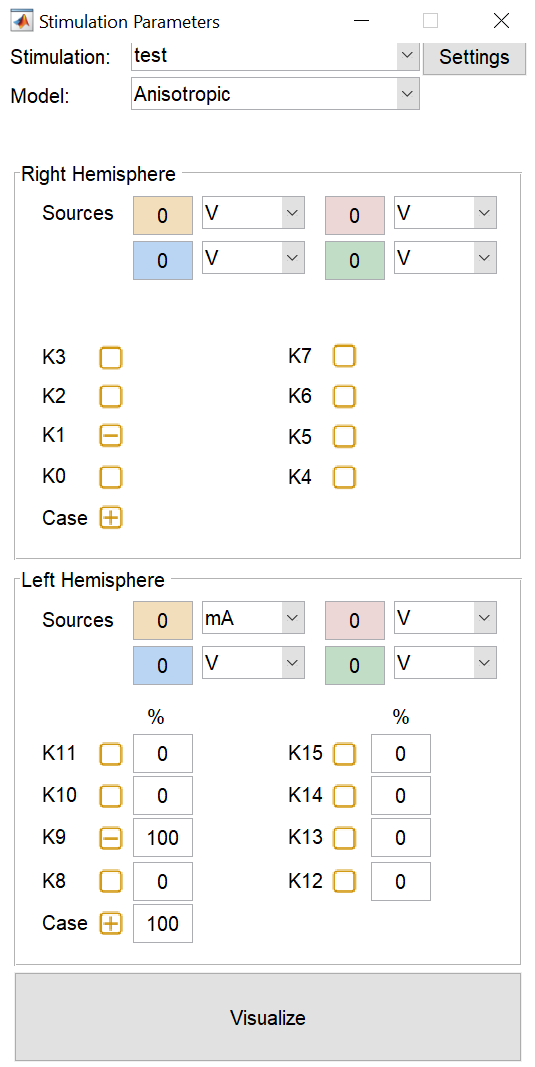
\includegraphics{images/stim.png}
	\caption{Stimulation Control Figure}
	\label{fig:stim}
\end{center}
\end{figure}

\begin{figure}
\begin{center}
	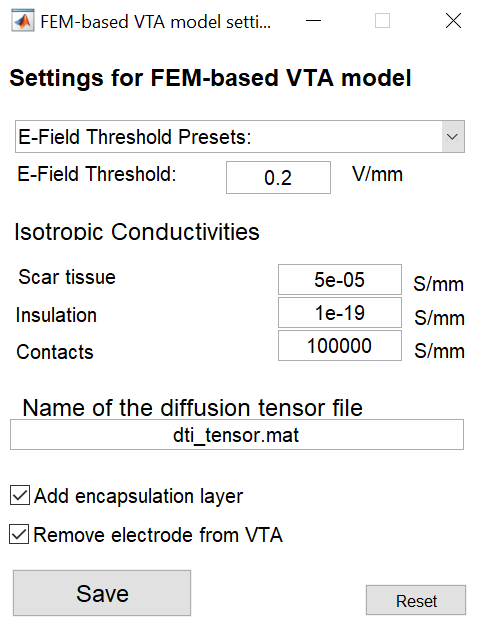
\includegraphics{images/settings.png}
	\caption{Anisotropic-model stimulation settings menu}
	\label{fig:settings}
\end{center}
\end{figure}

%__________________________________________________________________________________________________
\subsection{Output files}

The process also saves files which can be useful for further analysis. They are saved according to the directory hierarchy used by LEAD-DBS, which is 

\emph{<patient\_folder>/stimulations/<specific\_stimulation>}. If not specified, we assume their location is the one just described. These files are:

\begin{itemize}
\item \emph{stimparameters.mat}, which stores all the details regarding the way stimulation is applied;
\item \emph{mesh\_right.mat} and \emph{mesh\_left.mat}, which contain the data of the mesh for the right and left hemisphere respectively. They are directly stored in the \emph{stimulations} folder inside the patient directory;
\item \emph{conduction\_model\_right.mat} and \emph{conduction\_model\_left.mat}, which contain model of conduction for the right and left hemisphere respectively. They are directly stored in the \emph{stimulations} folder inside the patient directory as well;
\item \emph{vat\_right.mat} and \emph{vat\_left.mat} inside which we find a scalar representing the volume of the VTA in mm\textsuperscript{3}, a structure representing the mesh of the VTA and a structure containing information about the electric field and its gradient in the volume considered for VTA estimation
\item \emph{vat\_right.nii} and \emph{vat\_left.nii}, which are images representing the mask of the VTA in a region centerd in the middle of the VTA itself;
\item \emph{vat\_efield\_right.nii} and \emph{vat\_efield\_left.nii}, which contain the electric field in a volume centered in the middle of the VTA;
\item \emph{vat\_efield\_gauss\_right.nii} and \emph{vat\_efield\_gauss\_left.nii}, which contain the normalized electric field in the volume centered in the middle of the VTA.
\end{itemize}


\end{document}
